\chapter{System Specification}

\section{System Requirements}
\label{sec:require}
Before proceeding with the design and implementation of any software project it is important to define the requirements of the system to be developed. The requirements of a system define what the system must be able to do and are normally split into functional and non-functional requirements. Functional requirements of a system specify the explicit behaviour of the system and non-functional requirements specify other properties of the system that aren't explicitly related to the functionality, e.g. performance, file types supported etc.
\\In a professional software engineering environment the requirements gathering process would be conducted with the end user of the system, in order to ensure that what is developed matches what the end users actually want, and not what the developers think they might want. In this situation, a variety of requirement gathering techniques would be employed, some of which may include
\begin{itemize}
  \item{Document analysis; analysing any existing documents the end users currently use. This can help to establish the structure of database tables, or simply the datatypes the system should use}
  \item{Interviews. By interviewing end users, it is easy to get a list of what they want as well as an idea on how the system currently works}
  \item{Observation. By observing the current system, an idea of the flow of data etc. can be gathered}
  \item{Research. Research into the technologies available, or other similar solutions, can be a key factor in specifying a system}
\end{itemize}
Due to the nature of the project there is no specific end user, so the requirements were based on the research described in the previous section.

\subsection{Functional Requirements}
\begin{itemize}
  \item{The system must be able to play Connect 4 in The Arena as effectively as possible} 
  \item{The system must be able to optimise any unconstrained real valued maximisation or minimisation problem}
  \item{The system must optimise within the bounds defined by the problem only}
  \item{The system must implement the genetic, evolution strategies and particle swarm optimisation algorithms as described in the previous section}
  \item{The genetic and evolution strategies algorithms must be implemented supporting a number of the different selection and recombination methods described in the previous section}
  \item{The state of the system must be able to be written to and loaded from a file}
  \item{The system must store the fitness of each individual at each generation, and must allow this data to be plotted on a scatter graph}
\end{itemize}

\subsection{Non-functional Requirements}
\begin{itemize}
  \item{The parameters of the algorithms must be easily changeable} 
  \item{The system must allow new problems to be defined as easily as possible} 
  \item{The system must allow problem specific stopping criteria to be easily defined}
  \item{The system must allow new binary or real value coded population based algorithms to be added easily}
  \item{The system must be fully documented using JavaDoc}
  \item{The system must be machine and operating system independent}
\end{itemize}

\section{Development Methodology}
Using a software development methodology helps to keep any large scale development project in check. Development methodologies split development into a number of phases, which build on top of each other and guide the development of the software. Typical phases in a development methodology are analysis, design, implementation and testing.
\\The primary development methodology chosen for this project was phased development. In this methodology, the system is developed in phases of design, implementation and testing, with each phase building on the previous one, as shown by figure \ref{fig:phased}\cite{phased}. The use of this methodology is supported by the project's first and second aims. These aims can be used to split the project into two developmental phases; first, to develop a generic optimisation library and second to adapt this library to The Arena.
\begin{figure}[tp]
   \begin{center}
     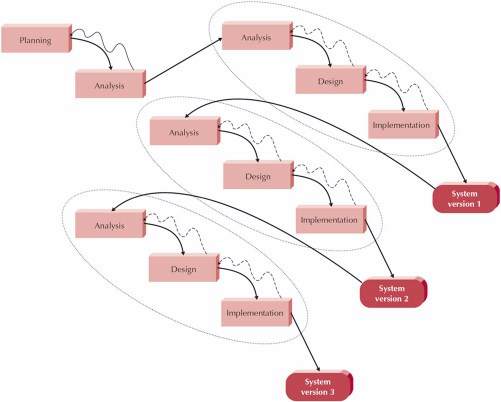
\includegraphics{Figures/phased}
   \end{center}
   \caption{Phased development methodology}
   \label{fig:phased}
\end{figure}

\subsection{Development Timescale}
Figure \ref{fig:gantt} shows the gantt chart of the planned development timescale. Following the end of phase two testing there is a testing phase during which the algorithms will be run, attempting to learn how to play Connect 4. As large period of time as possible, 4 weeks, was allocated for this, as it was unknown how long training would take when planning the project.
\begin{figure}[tp]
   \begin{center}
     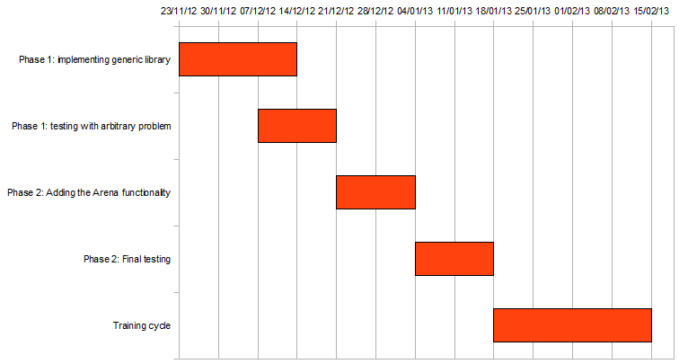
\includegraphics{Figures/gantt}
   \end{center}
   \caption{Gantt chart showing the development timescale}
   \label{fig:gantt}
\end{figure}